%!TEX root=./Emile.tex

\subsection[Spieltheorie]{Spieltheorie --- Was ist deine Strategie?}

\epigraph{
	``Gentlemen, Adam Smith needs revision.''
	\emph{John Nash}
	%MH TODO add correct reference
}

Die \emph{Spieltheorie} modelliert menschliche Interaktion in Form von Spielen, dessen \emph{Spielausgänge} von den gewählten \emph{Spielstrategien} abhängen und in Form einer Auszahlungsmatrix analysiert und veranschaulicht werden können \parencite[vgl.][153-274]{Kleinberg-2009-oz}.

\begin{quote}
	``Game theory is concerned with situations in which decision-makers interact with one another, and in which the happiness of each participant with the outcome depends not just on his or her own decisions but on the decisions made by everyone.''
	\parencite[vgl.][156]{Kleinberg-2009-oz}
\end{quote}

Bei einem \emph{Spiel} handelt es sich um eine Entscheidungsfindung von Spielern, in der alle Beteiligten wechselseitig von den Entscheidungen der anderen abhängig sind und stets nach Eigeninteresse handeln.
Ein Fallbeispiel für ein Spiel der Spieltheorie liefert das \emph{Gefangenendilemma}.

\begin{dsafigure}
	\begin{center}
	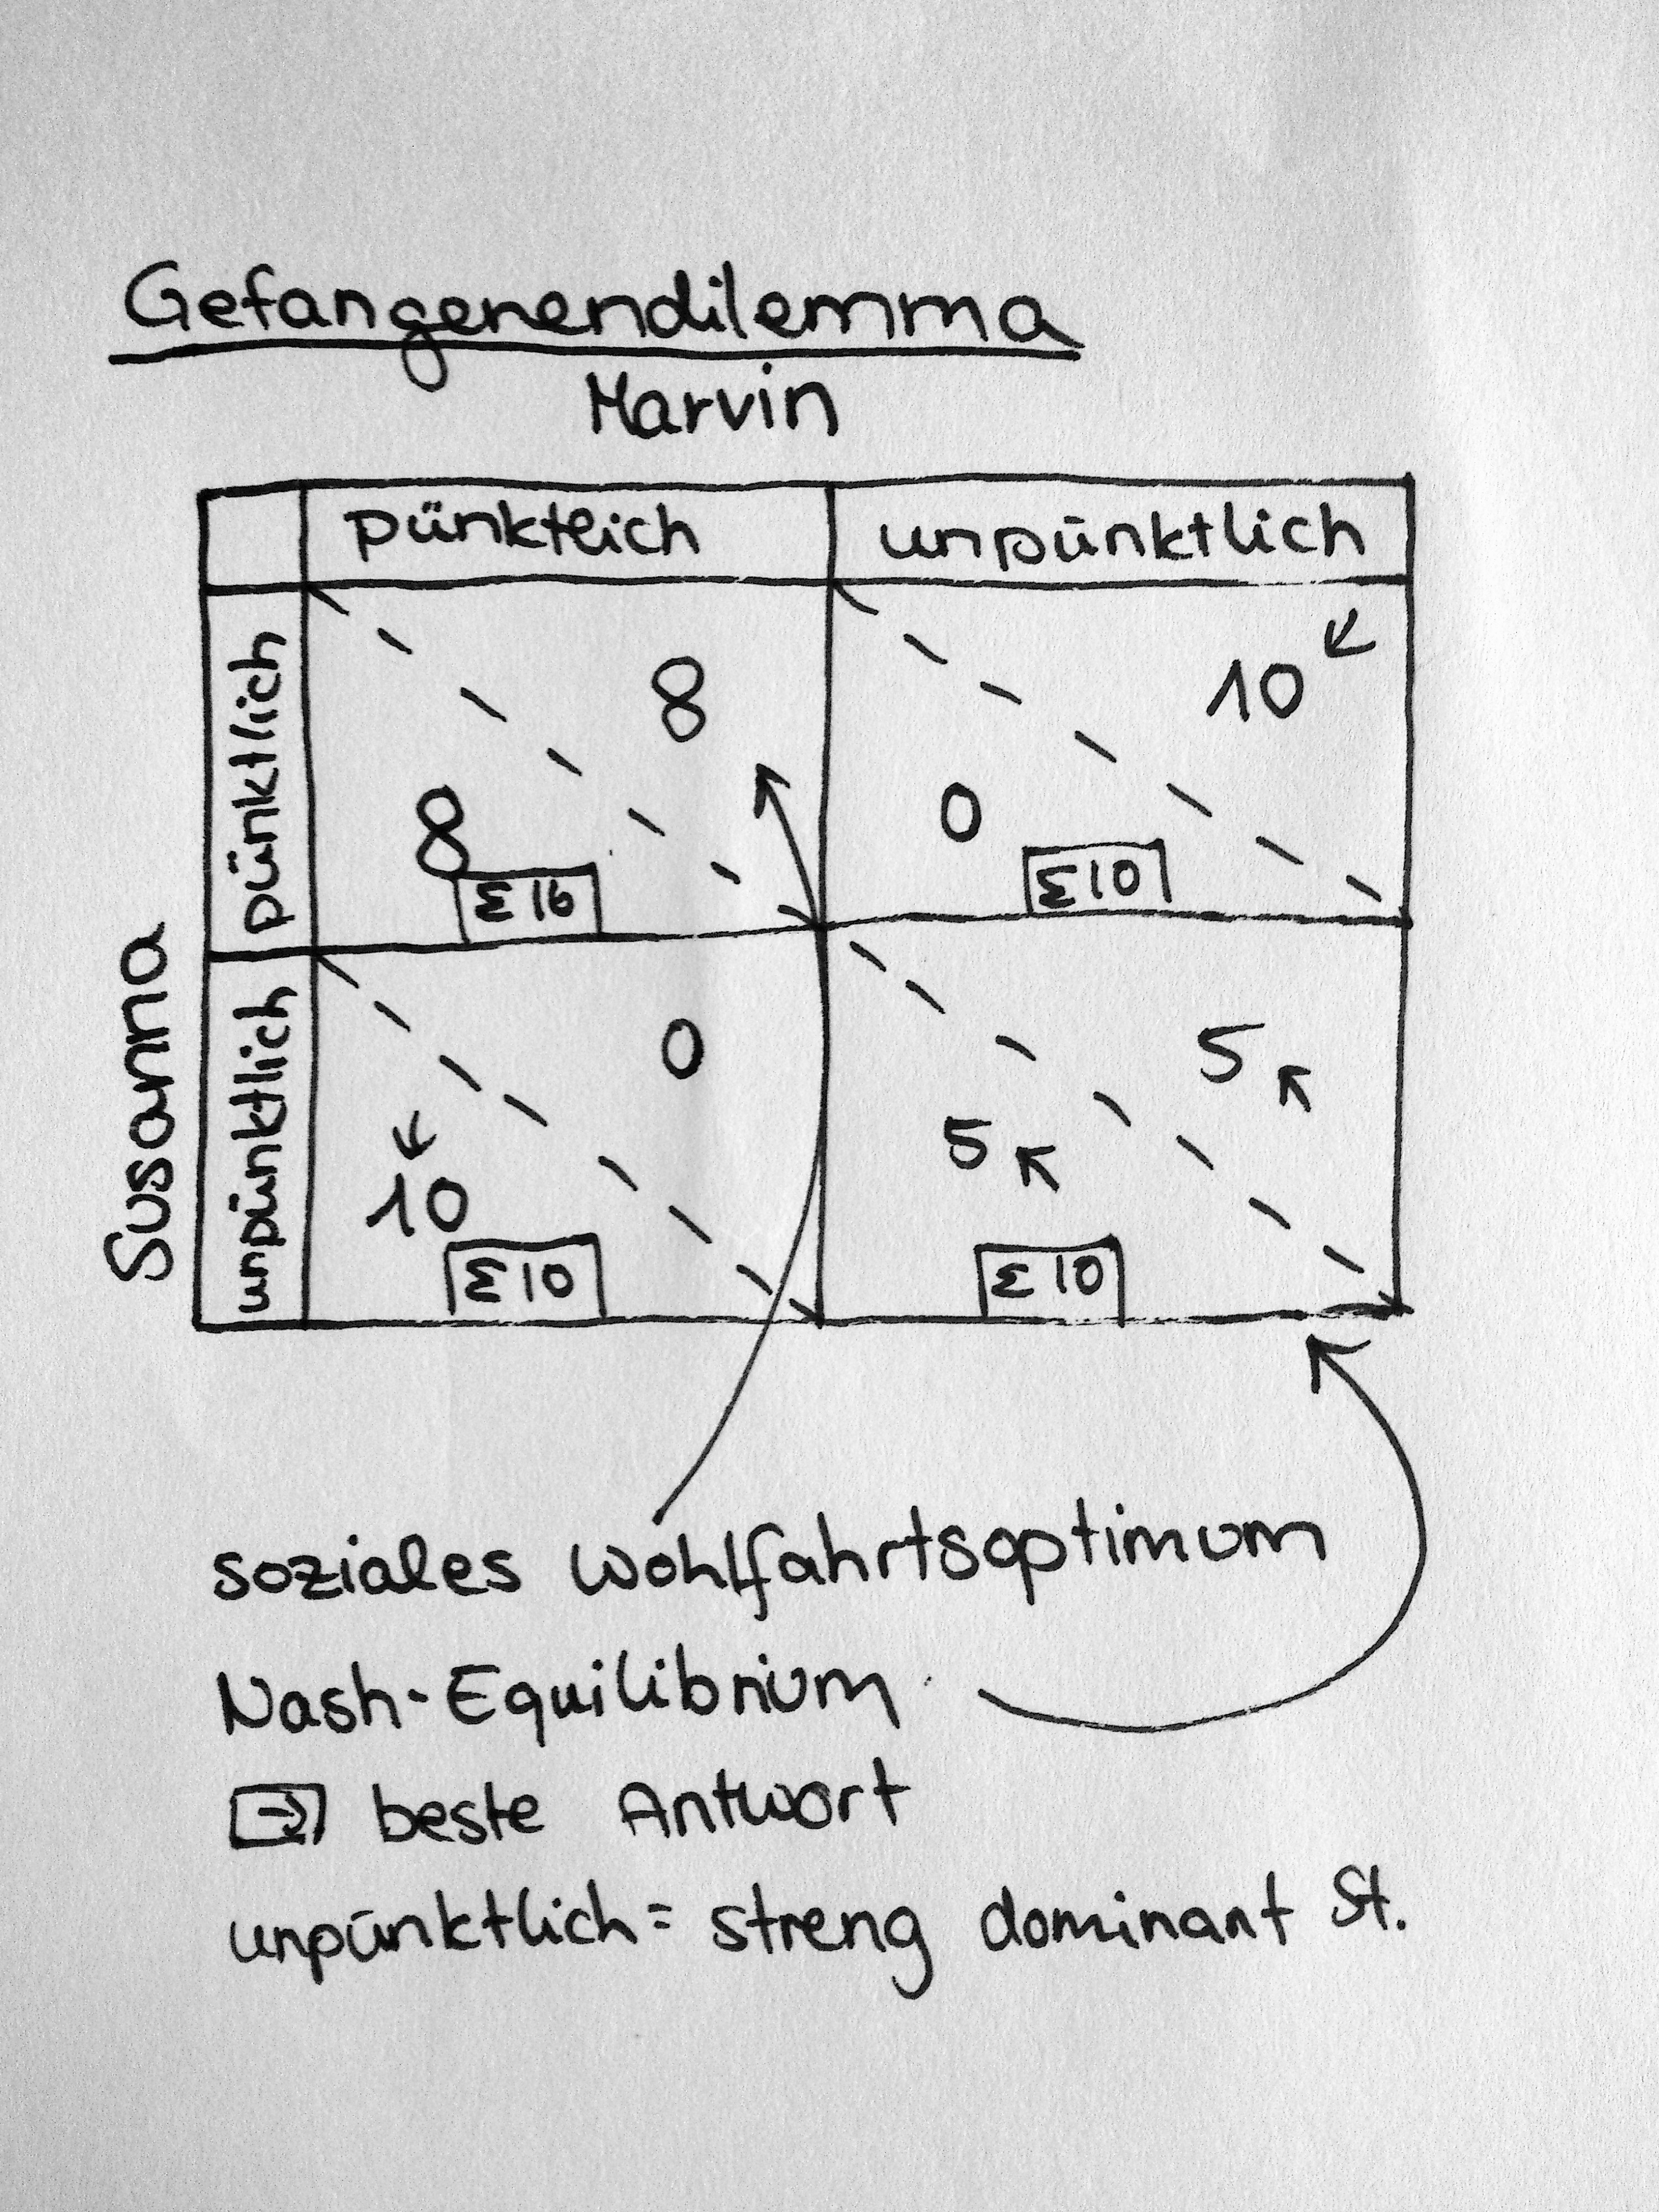
\includegraphics[width=0.9\columnwidth]{img/gefangendilemma.jpg}
	\caption{Beispiel für ein Gefangenendilemma nach \cite{Kleinberg-2009-oz}}
	\label{fig:gefangenendilemma}
	\end{center}
\end{dsafigure}

Die Abbildung oben stellt eine Auswahlmatrix dar.
Hier werden die Spielstrategien der Spieler dargestellt und die Summenanzahlen der Zellen in den jeweiligen Entscheidungen.
Verdeutlicht wird hier auch die wechselseitige Abhängigkeit beider Spieler: Wenn sich der Spieler (A/Marvin) für eine Spielstrategie entscheidet, so betrifft das auch Spieler (B/Susanna) und den Output beider Spieler.

Zum einem kann es \emph{Nullsummenspiele} geben.
Dabei haben alle Spielausgänge die gleiche Summen.
Es gibt lediglich Verteilungseffekte.
Zum anderen kann es \emph{Positivsummenspiele} (wie oben dargestellt) geben.
In einem Positivsummenspiel haben die Zellen unterschiedliche Summen. Unterschiedliche Spielausgänge führen also zu Wohlfahrtsverlusten oder -gewinnen.
Tatsächliche Kooperation -- also wechselseitig vorteilhafte Zusammenarbeit -- ist also nur bei Positivsummenspiel gegeben.
Demnach geben Nullsummenspiele keine Aussage über menschliche Kooperation, da die Summenanzahl bei jedem Spielausgang gleich bleibt.

\paragraph{Die Spielstrategien}

Eine Strategie gilt als \emph{beste Antwort}, wenn sie zu der Strategie eines anderen Spielers am besten passt, d.h. die eigene Auszahlung maximiert.
Hier sind mehrere beste Antworten möglich, wenn die Auszahlungen bei mehreren ``Antwort-Strategien'' gleich sind \parencite[vgl.][153]{Kleinberg-2009-oz}.

Eine Strategie ist \emph{streng dominant}, wenn der Spieler stets, unabhängig von den Mitspielern, die beste Auszahlung wählt \parencite[vgl.][164]{Kleinberg-2009-oz}.


\paragraph{Die Spielausgänge}

Ein \emph{Nash-Gleichgewicht } entsteht, wenn die die beiden Spieler Strategien gewählt haben, die jeweils die beste Antworten aufeinander sind.
Das \emph{soziale Wohlfahrtsoptimum} ist die Zellenkombination mit der höchsten Summe.

Der Erfolg einer Person im Spiel liegt somit nicht nur in seinen eigenen Entscheidungen, sondern darin welche Spielentscheidungen von allen anderen getroffen werden \parencite[vgl.][156]{Kleinberg-2009-oz}.


\paragraph{Die Axiome der Spieltheorie}

Nach Annahme der Axiome der Spieltheorie entscheidet sich der Mensch in seinem Handeln stets streng ökonomisch, das heißt, er verfolgt die Strategie mit dem größtmöglichen Gewinn.
Außerdem wird angenommen, dass jeder den \emph{Spielplan} kennt und somit auch alle Spielstrategien und Mitspieler.
Die letzte Annahme basiert auf der rationalen, indivduellen Nutzenmaximierung \parencite[vgl.][159]{Kleinberg-2009-oz}.


\paragraph{Die Spielvarianten}

Es ergeben sich auf diese Weise zwei möglich Spielausgänge von Positivsummenspielen:

\begin{enumerate}
	\item Spiele \emph{totaler Harmonie}: \emph{Zellen} von Nash-Gleichgewicht und Wohlfahrtsoptimum fallen hier zusammen. Das Nash-Gleichgewicht liegt im Wohlfahrtsoptimum.
	Beispielhaft ist für diesen Spielausgang ist der Handel.
	Die Annahme \emph{totaler Harmonie} im Handel würde auch Adam Smith unterstützen:

	\begin{quote}
		``Wer sein eigenes Interesse verfolgt, befördert das Wohl der Gesamtgesellschaft häufig wirkungsvoller, als wenn er wirklich beabsichtigt, es zu fördern. Ich habe nie erlebt, dass viel Gutes von denen erreicht wurde, die vorgaben, für das öffentliche Wohl zu handeln.'' \emph{Adam Smith ``Wealth of Nations''}
	\end{quote}
%VK: FIXME Richtigen Literaturverweis einfügen
	\item Spiele mit \emph{Kooperationsproblemen}: Summenanzahl von Wohlfahrtsoptimum und Nash Gleichgewicht unterscheiden sich.
	Ein Beispiel wäre das der Nationalen CO2-Emissionen. Entscheidet sich ein Land dafür, weniger Umweltschutzmaßnahmen zu treffen, so profitiert es davon nur, solange die anderen Ländern nicht die gleiche Strategie wählen.

\end{enumerate}

Beide Spielausgänge lassen sich in einem Baumdiagramm darstellen.

\begin{dsafigure}
	\begin{center}
	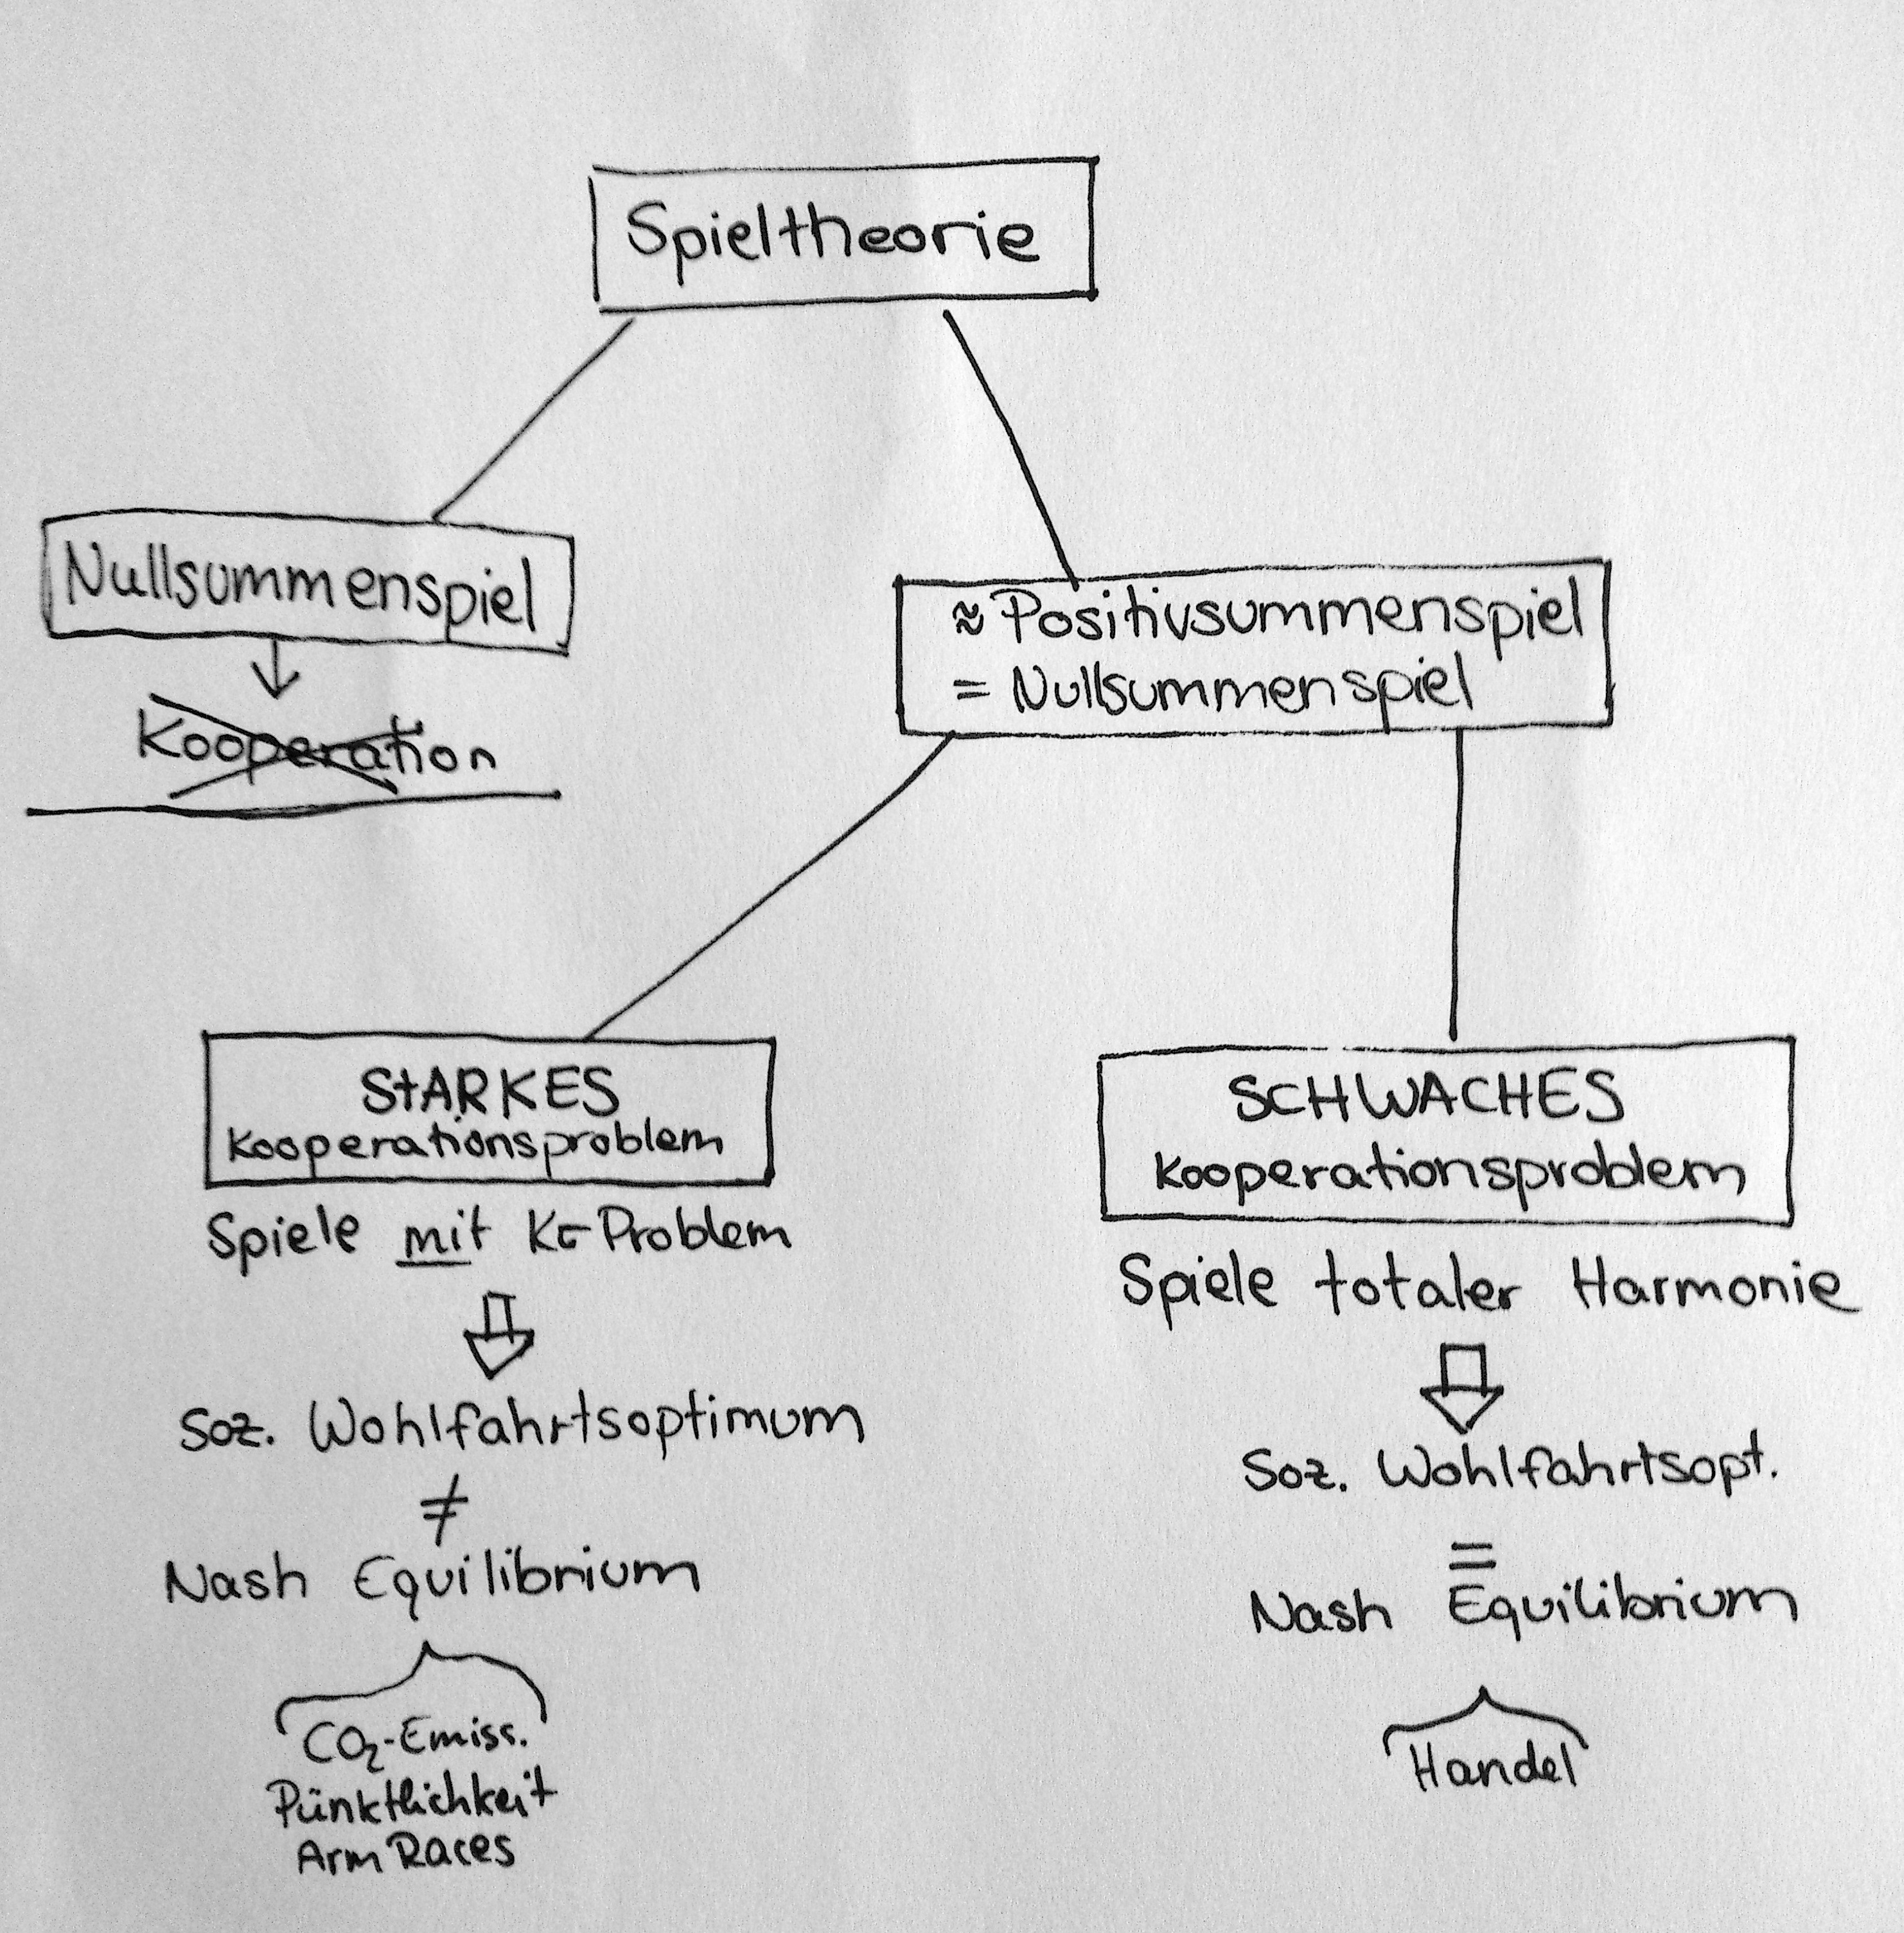
\includegraphics[width=0.9\columnwidth]{img/summenspiele.jpg}
	\caption{Summenspiele nach \cite{Kleinberg-2009-oz}}
	\label{fig:gefangenendilemma}
	\end{center}
\end{dsafigure}


\paragraph{Das Gefangenendilemma lösen}

Außer durch den Einfluss eines Gewaltmonopolists oder einer Änderung der Axiome, wie z.B. der Annahme des ``Gemeinwohls'' (vgl. \citeauthor{rousseau-1762}), kann das Gefangenen Dilemma nicht gelöst werden, da alle Spieler nur aus Eigeninteresse handeln.
Dieses Problem wäre durch Tillys Theorie der \emph{Staatsgenese} gelöst, sie stellt hierzu einen Gewaltmonopolisten bereit (vgl. \citeauthor{Tilly-1985-aa}).

Adam Smith lag somit mit seiner Annahme, dass die \emph{streng dominante} Spielstrategie stets auch am besten zum Allgemeinwohl beiträgt falsch, da man nicht grundsätzlich von Spielen mit \emph{besten Antworten} ausgehen kann und es dementsprechend, wie aufgezeigt, auch zu Kooperationsproblemen in menschlicher Interaktion kommen kann.


\paragraph{Anwendung der Spieltheorie}

Wie lässt sich die Spieltheorie in den Kurszusammenhang einordnen?
Das Modell der Spieltheorie stellt eine deutlich präzisere Formulierung des \emph{Kooperationsproblems} in der menschlichen Interaktion dar, indem es dieses auf ein mathematisches Modell zurückführt.
Durch diese Vereinfachung steht die Spieltheorie von Kleinberg aber auch in einem starken Kontrast zu dem Menschenbild der anderen Sozialwissenschaftler und Pädagogen, die wir im Kurs besprochen haben.
Kritisch zu hinterfragen ist, ob es sinnvoll ist, menschliche Kooperationsprobleme auf ein mathematisches System zurückzuführen beziehungsweise den Menschen durch Mathematik erklären zu wollen.
